
\subsection{地表水额度分配与灌溉需求的错配}

\begin{figure}[htb]
    \centering
    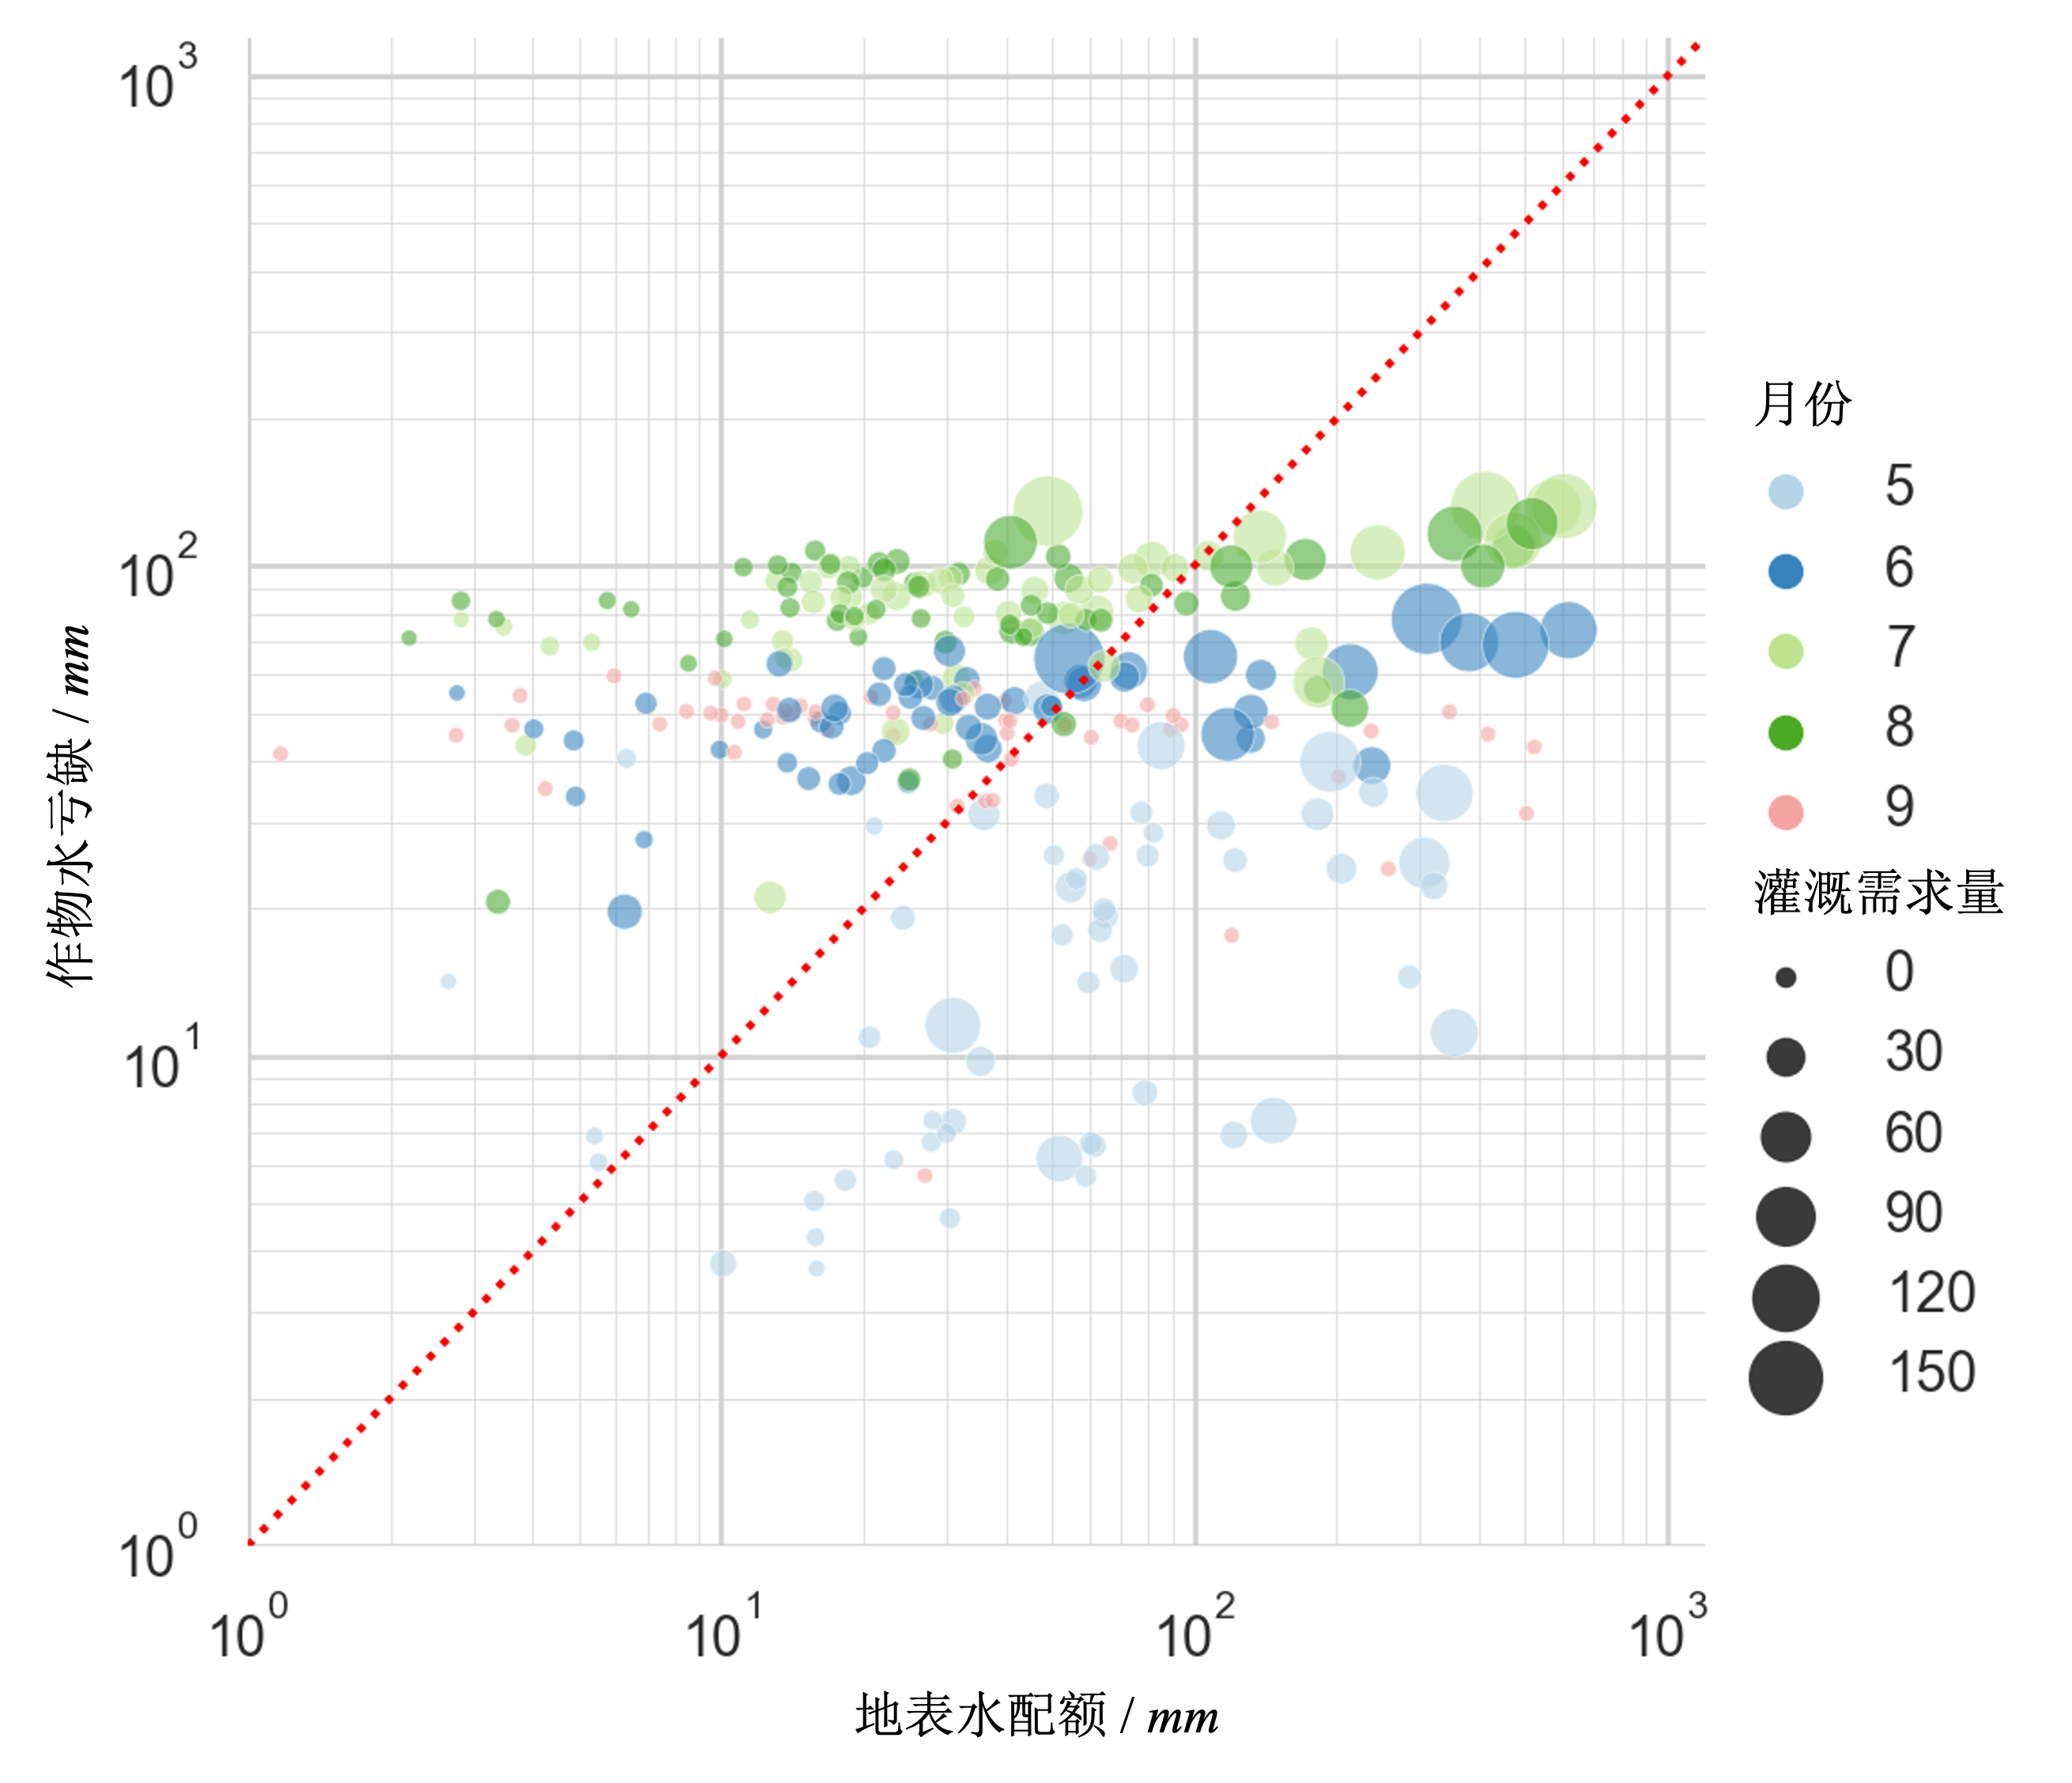
\includegraphics[width=0.8\textwidth]{img/ch6/ch6_matches.png}
    \caption{黄河流域地级市主要粮食作物生长季用水额度与用水需求的匹配情况}\label{ch6:fig:matches}
\end{figure}

在图\ref{ch6:fig:matches}中,展示了月尺度水资源配额与作物水资源亏缺的关系。红色虚线表示两者的$1:1$线,右侧表示配额大于作物需求,左侧则表示配额小于作物的绝对用水需求。研究发现,黄河地表水配额与水亏缺存在明显的时空分布不匹配现象。如果供给和需求匹配得很好,大多数气泡点应该落在$1:1$线上。然而实际情况是,气泡的大小代表了统计数据中的地区实际总灌溉用水量,可见水需求量较大的大型灌区也获得了较多的用水配额,容易出现配额供给大于实际作物需求的情况,而在规模偏小的地区则存在水配额供小于求的情况。
此外,气泡的颜色代表了作物生长季的不同月份,发现6月到9月之间的水资源供需失配情况分布比较相似,都是高需水地区有富余,低需水地区存在不足;仅在作物生长的初期(5月)的配额普遍出现水资源配额富余的情况。

\begin{figure}[htb]
    \centering
    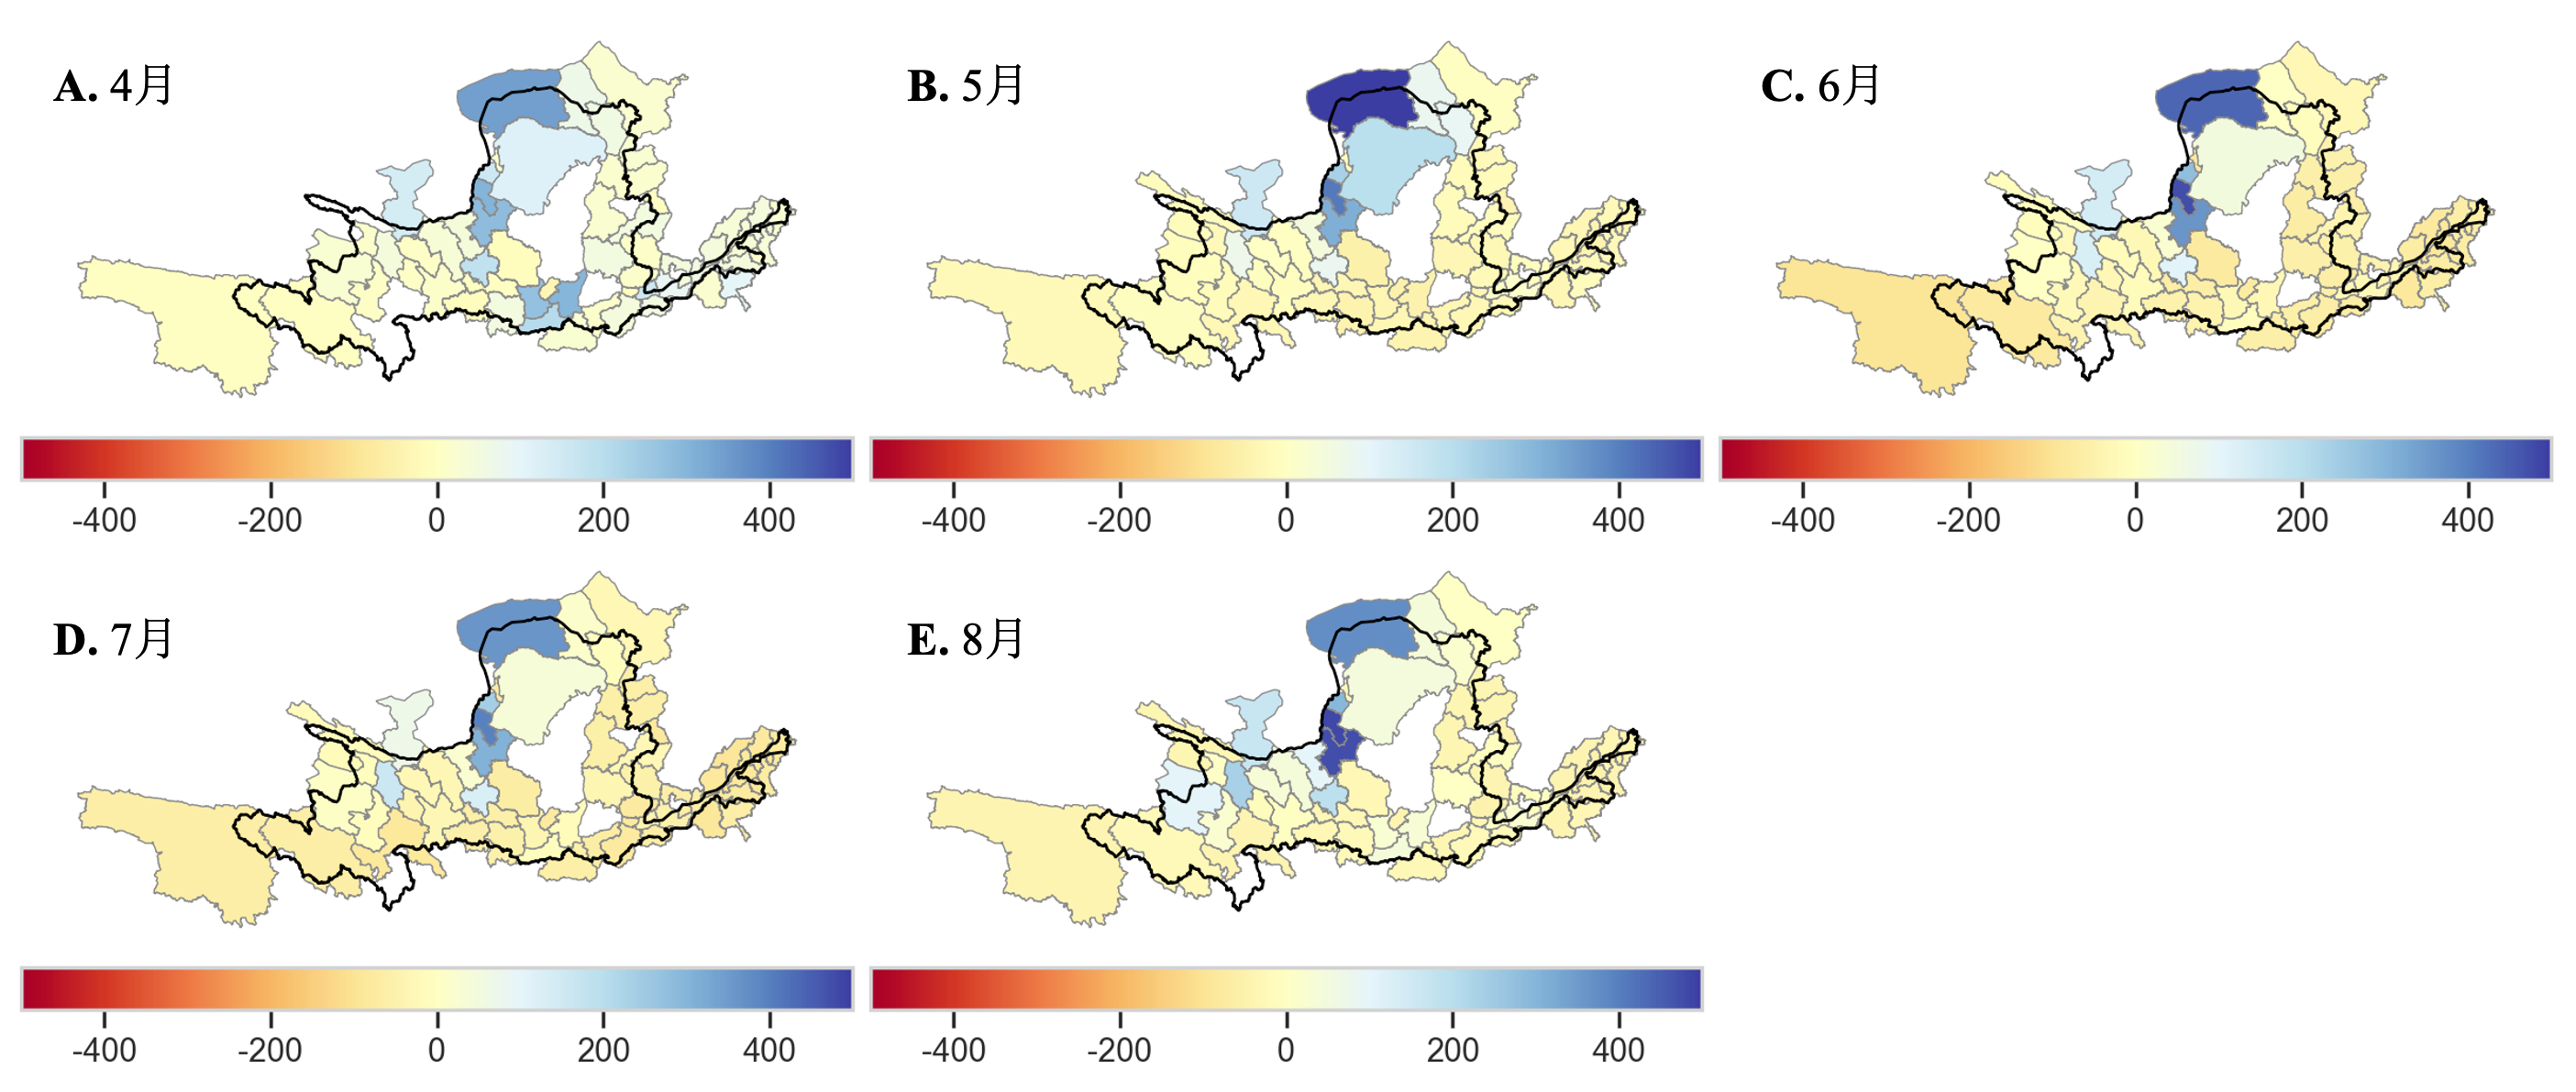
\includegraphics[width=\textwidth]{img/ch6/ch6_deficits_map.png}
    \caption{主要粮食作物生长季黄河地表水配额与作物需水量之差}\label{ch6:fig:deficits_maps}
\end{figure}

进一步将两者差值映射到空间上,如图\ref{ch6:fig:deficits_maps}所示,可以发现五月的配额大多数地区属于供需平衡的状态,而七、八月的供需匹配情况更为严重,作物需求和配额供给之间的差异部分地区有超过$500mm$的配额富余,但其它地区则平均有超出$100mm$的配额缺口。
在各个月份中,配额富余主要分布在宁夏和内蒙古的河套灌区,这在六月尤其明显;而下游山东灌区则在除五月之外的生长季均有严重的配额不足情况。

\subsection{用水者决策对分水制度变化的响应}

\begin{figure}[htb]
    \centering
    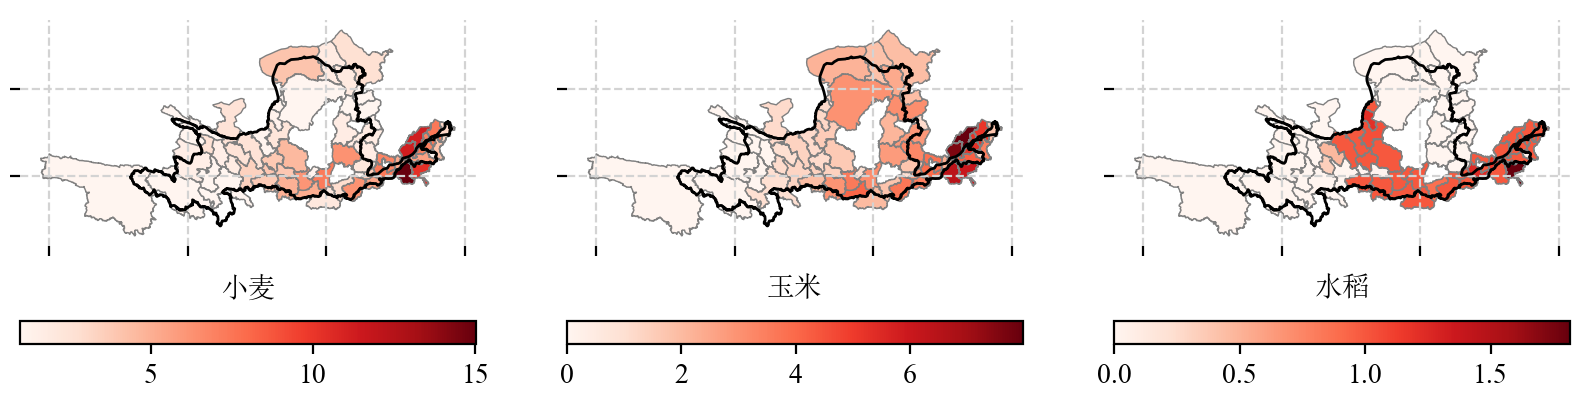
\includegraphics[width=\textwidth]{img/ch6/ch6_agents.png}
    \caption{黄河流域主要粮食作物的三种主体平均分布数量}\label{ch6:fig:agents}
\end{figure}

本研究根据灌溉面积生成各类粮食作物灌溉主体数量,水稻、玉米、小麦三类主体的数量分布如图\ref{ch6:fig:agents}所示,小麦种植面积最广,玉米其次,水稻仅部分地区有少量分布,地级市尺度上平均生成的主体数量不足$2$个。
将$1987$年“八七”分水方案出台后的每三年分成一个时间段,将此地表水配额灵活时期分为初期($1988 \sim 1991$)、中期($1992 \sim 1994$)、后期($1995 \sim 1998$)三个时段,诸省份农业主体在不同时期对水资源配额的合作比例如图\ref{ch6:fig:compliacne}所示。
由于社会系统存在决策的演化传播,违背分水制度进行超额取水的主体比例会随时间变化,大多数省份的主体的变化趋势都是在初期到中期合作比例显著下降,在中期到末期又显著上升的“V”形变化趋势。
整体来说,大多数省份在$1987$年“八七”分水制度出台后的十年时间里都偏向于违背此分水配额。
% 且会随两个人类模块的参数$b$和$v$(见表\ref{ch6:tab:params})的取值变化存在阈值效应。
在三种主要粮食作物中,种植水稻的主体对制度变化的响应更为敏感;种植玉米的主体在中期至后期合作的比例趋于稳定;种植小麦的农户违背配额政策决策的占比则持续增加。


\begin{figure}[htb]
    \centering
    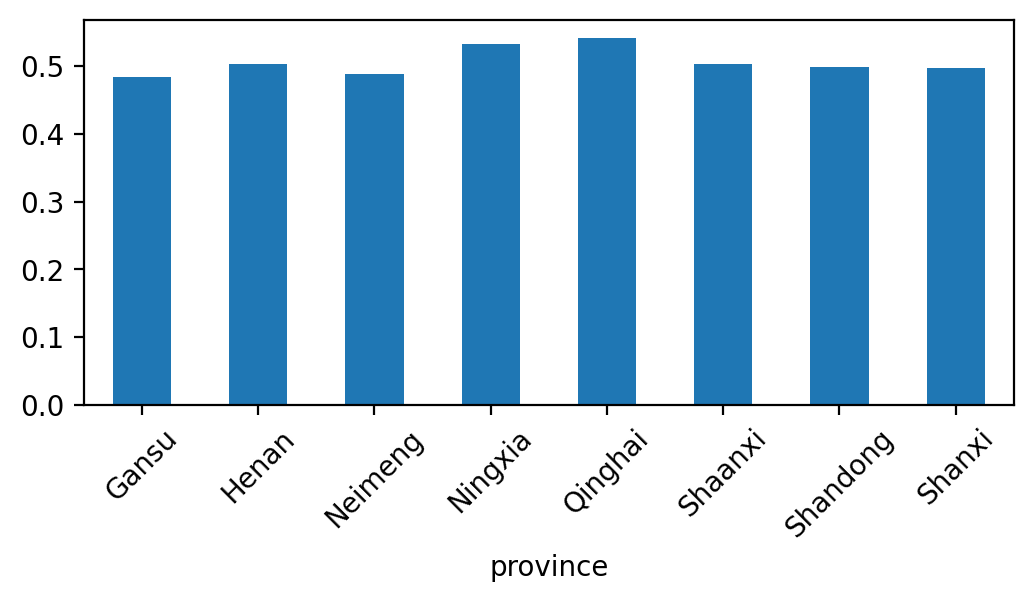
\includegraphics[width=\textwidth]{img/ch6/ch6_compliance.png}
    \caption{“八七”分水方案颁布至流域统一调度开始之前主体博弈决策中选择合作的比例}\label{ch6:fig:compliacne}
\end{figure}

\subsection{用水来源受分水制度变化的影响}

本研究所建立的模型可以模拟黄河流域主要粮食作物种植中各类水源(降水、地表水、地下水)的使用情况。研究发现,天然降水是黄河流域大多数省份粮食作物生长的主要水源。然而,在河套灌区的宁夏和内蒙古两自治区,地表水灌溉的占比更大(见图\ref{ch6:fig:sources})。此外,各省总体上都保持了蓝水使用占比持续下降的趋势,但是对用蓝/绿水比例的影响并不明显,仅青海和山西存在一定程度的突变。
另外,通过分析地表水和地下水的使用量,发现地表水使用量前$50\%$的主体在$1987$年到$1998$年之间用水量进一步扩大,而另外$50\%$用水量较小的地表水使用量则仍分布在约$100mm$以下。同时,地下水和灌溉用水的分布则在两次分水制度前后变化不大,如图\ref{ch6:fig:sources_change}所示。


\begin{figure}[htb]
    \centering
    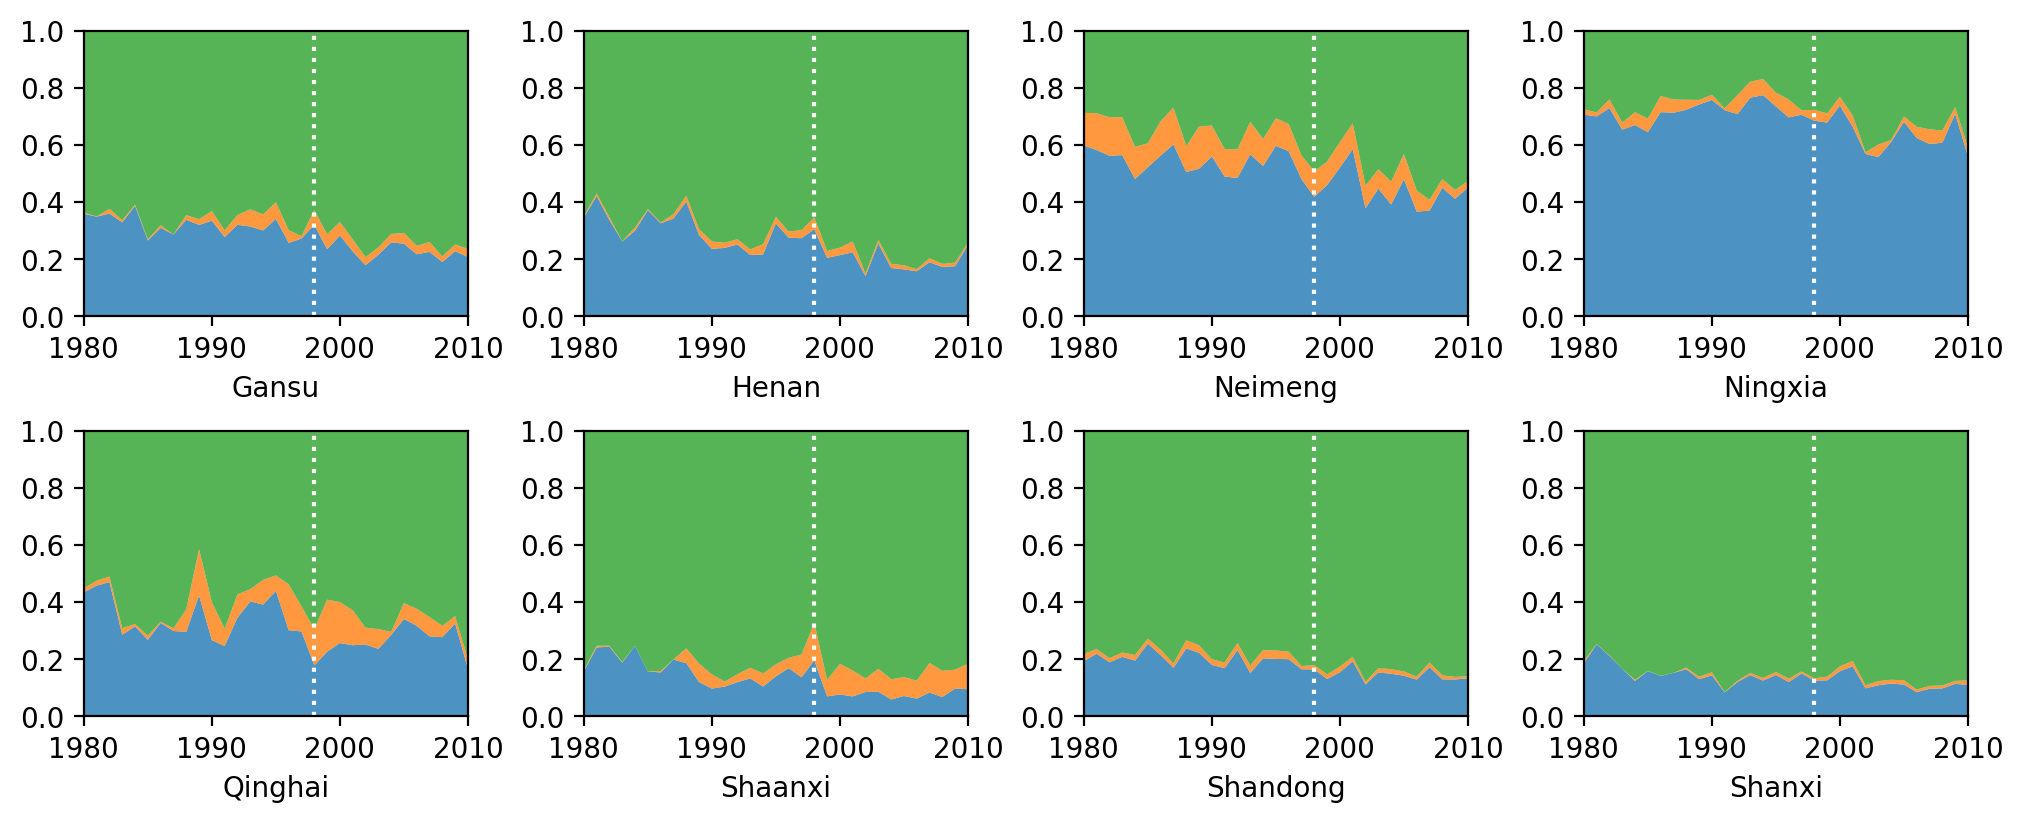
\includegraphics[width=\textwidth]{img/ch6/ch6_green_blue_water.png}
    \caption{黄河流域主要农作物用水来源的比例变化}\label{ch6:fig:sources}
\end{figure}

\begin{figure}[htb]
    \centering
    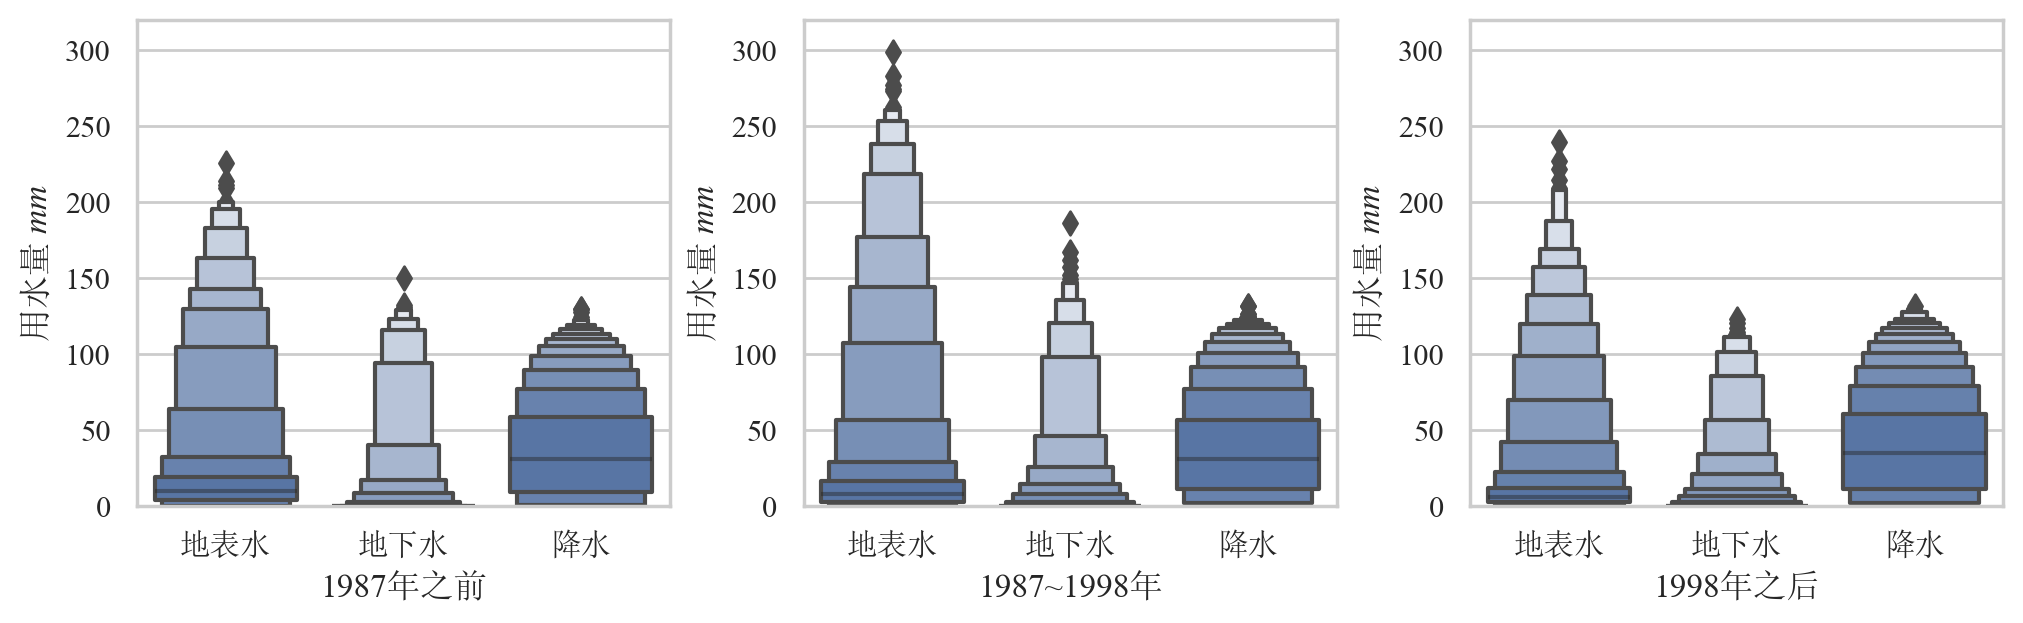
\includegraphics[width=\textwidth]{img/ch6/ch6_sources_change.png}
    \caption{黄河流域分水制度变化前后的用水来源比例统计}\label{ch6:fig:sources_change}
\end{figure}

地下水使用量是分析黄河流域分水制度变化影响的重要指标。研究表明,分水制度变化对黄河流域的地下水使用量带来的影响较为明显。
具体来说,中游地区持续增加地下水的开采量。
而上游和下游地区在1987年分水制度提出之初期先加大了地下水的开采量,在1998年统一调度制度实施后才大力推行节水改革。

\begin{figure}[htb]
    \centering
    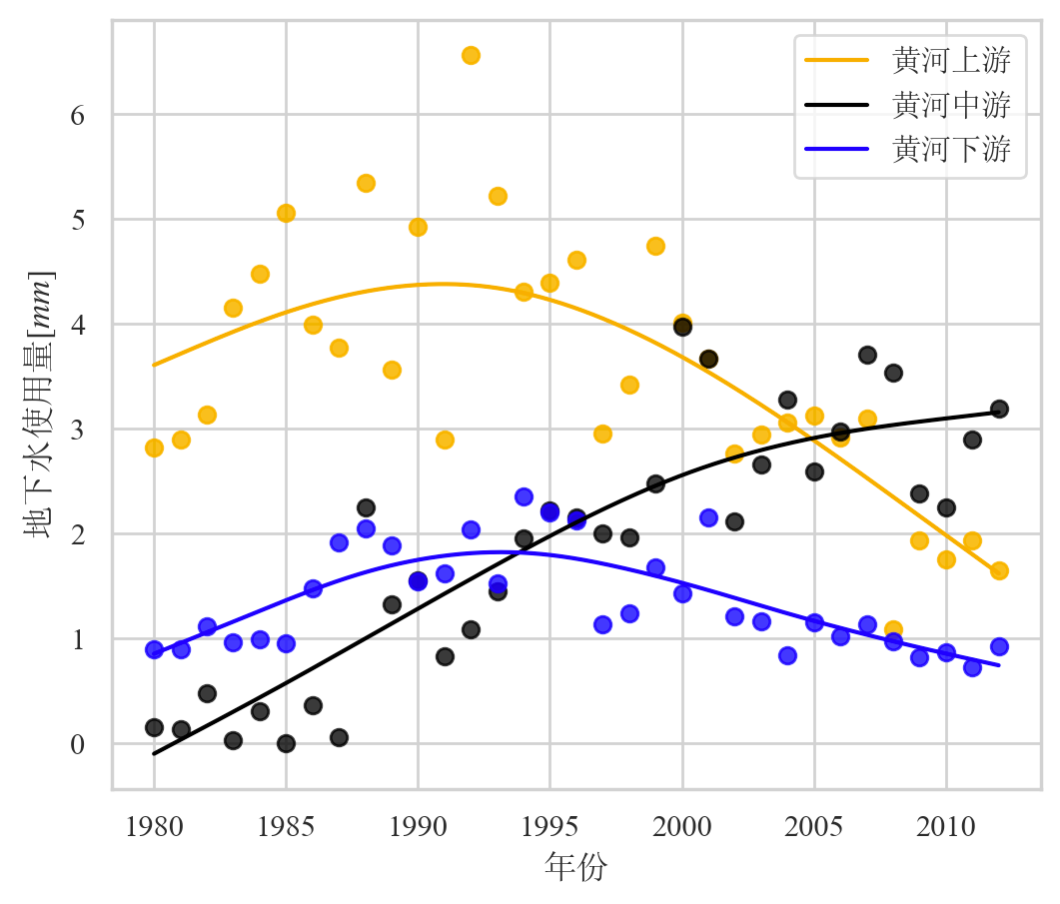
\includegraphics[width=0.6\textwidth]{img/ch6/ch6_groundwater.png}
    \caption{黄河流域、中、下游地下水开采量对分水制度变化的响应}\label{ch6:fig:groundwater}
\end{figure}